\chapter{Literature Survey}
%wide context
%detailed context
%recent work 
%    critically assess previous work
%questions and issues that have not yet been answered

\section{Speech Prosody}
In linguistics, prosody as a terminology refers to the suprasegmental information in speech comunication. It is mainly characterized by varibles including the fundamental frequency (f0), the duration and the energy of the sound. F0 exhibits the frequency of vibration of the vocal folds; the duration is defined from a phonetic segmentation of the speech signal; The energy, or intensity, refers to raw local energy of the spoken utterance. Being suprasegmental means that prosody is defined on segments larger than the phones.

prosody conveys various types of linguistic information over the spoken utterance. For example, prosody plays a similar role in structuring spoken message as punctuation does in written texts; and emphasize the important part of the message for a easier delivery to the listener. The use of prosody can also reflect the attiutude and emotion of the speaker. \citep{Jurafsky2008, Hirschberg2017, Jouvet2019}

The study of prosody is fundamental to both basic research and applications in speech and natural language processing. Prosodic cues have been applied to many fields of language technology, especially speech synthesis  \citep{Schuller2018}, automatic summarization \citep{Chen2010} and emotion detection \citep{Liu2016} in spoken utterances. 

 
%\subsection{Prosodic analysis}
%Prosodic analysis aims to compute an abstract representation of the prosodic prominence, structure and tune of the spoken utterance.
%
%Most of the previous study focuses on the prosodic structure, prosodic prominence, tune and the use of features including pitch, energy and duration \citep{Pierrehumbert1980,Pierrehumbert1990,Pierrehumbert2015,Hirschberg2002}. 
%
%Recently, researchers explored vector representation of words based on speech and its prosodic features \citep{He2016, Chung2018}, a similar approach as the widely used word embedding technique "word2vec" in Natural Language Processing.     
%
%\subsubsection{Prosodic Structure}
%Similar to the grammartical structure of a written sentence, spoken utterances have such a structure as some words group naturally together and form a boundary or break. There is a term to describe prosodic structure--prosodic phrasing. A spoken sentence could be divided into intonational phrases, those separated by commas in text, and even smaller units called intermediate phrases. 
%
%Prososic phrasing is of great use in tasks such as speech synthesis. Automatic phrase boundary detection can be regarded as a classification problem. 

%\subsubsection{Tune}
%The tune of an utterance is the rise and fall of its $F_0$ over time. The typical tunes in English are a rise of the voice at the last word in a yes-no question and a drop at the end of a statement. The former is called the question rise and the latter the final fall. 
%
%The tune is a useful facility to express meaning and emotions. It can be inferred from the tune contour that whether the speaker is surprised or in a contradiction. For a long time, most of the systems are only able to distinguish two or three tunes yet more and more work emerges on this topic.

\subsection{Prodody: Analysis and Models}
One of the ultimate purpose of studying prosody is to gain a knowledge that is sophiscated enough to allow precise predictions of prosodic patterns. Prosody analysis and the computational modelling of prosody are two driving forces interacting with each other towards our ultimate goal with gradual progressions. \citet{Xu2015} summarises in his overview of prosody researches that despite various disputes between theories and models of prosody, there is a clear historical trend toward approaches that are hypothesis-driven, experimental-based, detail-sensitive, and modeling-oriented. What is underlying is drive to achieve predictive rather than merely descriptive knowledge of prosody. 

This is seen in the gradual progression through research strategies that may be characterized as analysis by introspective transcription, analysis by acoustic transcription, analysis by hypothesis testing and analysis by modeling (Xu, 2011). 

The early days of prosody research was dominated by descriptive methods that can be collectively characterized as analysis by introspective transcription. In this approach, symbolic representations of prosodic events are proposed based on the researcher’s intuition and nonexperimental observation. Crystal (1969)

In this tradition, intonation is portrayed by a transcription system consisting of representations for prominences (usually by the size of successive dots corresponding to the stressed syllables) and contours (by curved lines, sometimes with arrow heads to indicate the direction of pitch movements), as illustrated in the top panel of Figure 2. transcription systems in America that emphasize tonal levels rather than tonal contours. An apparent issue with this general approach is that human
introspection about prosody is not highly reliable.

This situation has been significantly improved over the years thanks to the availability of various hardware and software tools. This has led to the development of a new approach, namely, analysis by acoustic transcription.

One of the best-known systems in this approach is Tones and Break Indices (ToBI) (Silverman et al., 1992). The system is developed based on the pitch accent representations proposed by Pierrehumbert (1980) and the boundary representations proposed by Price et al. (1991). 

directly observable, 

In more recent research, analysis by acoustic transcription is incorporated into some empirical studies, in which the transcriptions are used as measurements and subjected to statistical analysis
the hypothetical nature of the categories in the transcription systems themselves, which can be questioned if the experimental results fail to provide support. 

Neither the hypotheses nor the predictions are considered as corroborated until there is sufficient experimental support. And, even with strong corroborations, the prosodic categories themselves are not treated as part of the indispensible core of a theory, as in the case of the analysis by transcription approaches.


%\subsection{Tone and Break Indices Model: ToBI}
%ToBI (Tone and Break ToBI Indices) is the dominant linguistic model for describing prosodic features in American English speech utterance \citep{Silverman1992, Pitrelli1994}. It models boundaries, prominence, tune based on the 4 boundary tones and 5 pitch accents shown in the following table.
%
%%(insert table here)
%\begin{figure}[ht]
%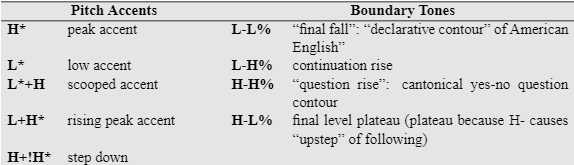
\includegraphics[width=15cm]{figures/ToBI_1.png}
%\caption{The accent and boundary tones labels from the ToBI transcription system Reproduced from D. Jurafsky and J.H. Martin, 2nd\_ed\_draft: Speech and Language Processing with the permission of the copyright owner.}
%\label{fig:ToBI1}
%\end{figure}
%
%In ToBI, an input utterance is represented by a sequence of intonational phrases and intermediate phrases. The intonational phrases end in one of the four boundary tones which describe the tune. Each word in the utterances will be assigned a pitch accent of the five types. Furthermore, ToBI adopts a separate break index tier to distinguishes four levels of phrasing: break index4-intonational phrase; break index 3-intermediate phrase; break index2-disjuncture or pause; break index 1--medial word boundaries \citep{Hirschberg2002}.
%
%%(insert figure here)
%
%\begin{figure}[ht]
%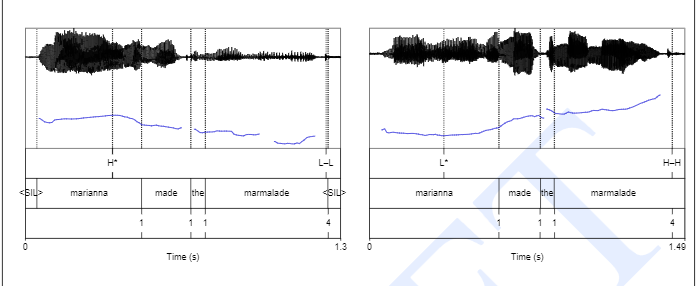
\includegraphics[width=15cm]{figures/ToBI_2.png}
%\caption{An example of ToBI discription, Reproduced from D. Jurafsky and J.H. Martin, 2nd\_ed\_draft: Speech and Language Processing with the permission of the copyright owner.}
%\label{fig:ToBI2}
%\end{figure}
%
%One goal of ToBI is to display the link between meanings and pitch accents. With the Praat program, we are able to visualise the tone, orthographic, and phrasing tiers of a ToBI transcription. In (a), the word Marianna is spoken with a high $H^*$ accent, and the sentence has the declarative boundary tone L-L\% whereas in (b) the same word is spoken with a low $L^*$ accent implying a surprise emotion. In addition, boundary tone H-H\% in (b) follows the yes-no question pattern \citep{Pitrelli1994, Jurafsky2008}. 

\subsection{Prosodic Prominence}
When a speaker says some words with a raised voice, slower pace or with more energy, the listener seems to feel these words are more prominent or important. Pitch accent and stress are the linguistic markers used to denote a prosodic prominence. Most of the content words are accented whereas function words tend not to bear pitch accent. Generally speaking, more informative words (for example new words or unexpected words) are more likely to bear accent \citep{Beckman1986, Bagshaw1994}.

Previous literature examines the relationship between prosodic prominence and accoustic features: pitch accents are suggested to be closely connected with fundamental frequency (F0) movements and syllable overall energy \citep{Bagshaw1994, Streefkerk1999, Brenier2005}; and stress shows a strong correlation with syllable nuclei duration and mid-to-high-frequency emphasis\citep{Sluijter1996, Tamburini2003}. Such acoustic correlates have been adopted to build automatic prosodic prominence detection systems\citep{Tamburini2003}. The number of syllables spoken in a word can also be estimated using the \citet{DeJong2009} model. 

%http://ec-concord.ied.edu.hk/phonetics_and_phonology/wordpress/learning_website/chapter_1_introduction_new.htm#1.2.1

%\section{applications}
%Previous researchers have modeled prosodic
%cues in speech for various applications (Tran et al., 2017; Brenier et al., 2005; Xie et %al., 2009). 
%
%For instance, in automatic prominence detection, re- searchers predict regions of speech %with relatively more spoken stress (Wang and Narayanan, 2007; Brenier et al., 2005; %Tamburini, 2003). Identifi- cation of prominence aids automatically identify- ing content %words (Wang and Narayanan, 2007), a crucial sub-task of spoken language understand- ing %(Beckman and Venditti, 2000; Mishra et al., 2012). 
%
%Moreover, researchers have investigated modeling prosodic patterns in spoken messages to %identify syntactic relationships among words (Price et al., 1991; Tran et al., 2017). In %particular, (2017) demonstrated the effectiveness of speech- based features in improving %the constituent pars- ing of conversational speech texts. In other work, researchers %investigated prosodic events to iden- tify important segments in speech, useful for pro- %ducing a generic summary of the recordings of meetings (Xie et al., 2009; Murray et al., %2005).

\section{Word Predictability}
In lauange engineering, the task to predict a word based on the given information is called language modelling. Lanugae models are ubiquitous in the field of natual language processig, notablly in machine translation, text summarisation, recommendation systems and other scenarios. It also plays an essential role in automatic speech recognition. Researchers care about word preditability as a major measurement to evaluate the performance of many autimatic systems. Word predictabity is supposed to be closely related to the amount of impormation that the word conveys, which is partiallly reflected by measurements such as perplexity, term frequency inverse document frequency (TF-IDF) value and some human-anotated word importance scores.

%Given the close relation between prosodic prominence and word importance, the description and application of prominence requires semantic knowledge. Features such as TF-IDF, part-of-speech and accent ratio are usually adopted to predict accents.

\subsection{Perplexity}
Perplexity (denoted by $PP$ for short) is the most common evaluation metric to test how well a statistical language model matches a test corpus.  For a test set $W = {w_1, w_2, \cdots, w_N}$ where $w_i$ is a sentence in the set, the perplexity is the probability of the test set, normalized by the number of words \citep{Jurafsky2008}:

\begin{equation}
PP(W) = P(w_1, w_2, \cdots, w_N)^{-\frac{1}{N}}\\
= \sqrt[N]{\prod_{i=1}^{N} \frac{1}{P(w_i|w_1, w_2,\cdots, w_{i-1})}}
\label{eq:perplexity}
\end{equation}

It is assumed that a better language model will assign a higher probability, or higher maximum likelihood to a sentence of the test set hence the perplexity will be lower. Examining perplexity on word level, threre is another interpretation that the perplexity of a word is defined by how many possible words the model has as candidates to make the prediction.

\subsection{TF-IDF}
Apart from the raw probability of a word in a corpus ( computed based on term frequency ), a more advanced weighting scheme named Term Frequency - Inverse Document Frequency (TF-IDF) is also widely to express the imformative feature of the word. Given a corpus with $D$ documents, the term frequency of a word $N_w$ means the number of appearance of a word $w$ in a particular document $d$. Document frequency indicates that there are $k$ documents in the corpus, which contain the certain word $w$. In practice, we use the inverse document frequency times term frequency to capture the semantic importance of a word in the context of that corpus \citep{Jurafsky2008}.

\begin{equation}
TF*IDF(w) = N_w \times \log(\frac{D}{k})
\label{eq:tf-idf}
\end{equation}


\subsection{Word Importance}
When it comes to words, we intuitively feel that some words are more importance than others no matter in reading or in conversation. Researchers in Psychology have used eye-trackers to study reading behavior. They found that readers tend to skip words, gaze on a word or glance back at previous words instead of reading very word in a text sequentially. It indicates that some words seem more important than others and words which are often skipped over by the readers tend to be shorter and more predictable \citep{Rayner2011}. 

Is word importance quantilisable? From previous sections, we can see that probability, perplexity and TF-IDF of a word do cast some light on the numeric representation of word importance. Moreover, researchers have developped resources of word importance scores determined by human annotators \citep{Kafle2018}. 
 
Prior researches on identifying and scoring important words in a text basically focused on the task of keyword extraction and document automatic summarisation. Metrics of word importance been explored include TF-IDF weighting \citep{HaCohen-Kerner2010}, word co-occurrence probability estimation \citep{Y.MATSUO2004} as well as other linguistic features investigated with supervised learning methods \citep{Liu2011, I.Sheeba2012, Murdoch2018}. 

\subsection{Prosody and Word}
There are researches investigating the relation between prosody and word. Similar to the approach of word-embedding \citep{Mikolov2013}, i.e., representing a word with an multi-dimensonal vector ), scholars have investigated encoding semantic properties of a word directly from speech \citep{Chung2018}. Lexical and prosodic cues have been intergrated to help listeners disambiguate difficult parses\citep{Tran2018}.

As for word importance, \citet{Kafle2019} developed a model to learn a word-level representation from prosodic features at a sub-word level for the task of importance prediction in spoken dialogue. Using software tool Praat (introduced in Section) they extracted 30 features in total: 3 voicing features, 6 spoken-lexical features, 10 pitch-related features and 11 energy features. These features also got speaker-normalized (ZNORM). Their work proves that using only acoustic prosodic cues, a automatic word importance detection system could yield comparable results to models based on texts.

\section{Correlation}
In statistics, there are many tools to describe the relationship between pairs of variables. Two variables are related if pairs of scores show an orderliness that can be depicted graphically with a scatterplot and numerically with a correlation coefficient.

\subsection{Pearson Correlation Coefficient}
Pearson Correlation Coefficient (r) is a number between –1.00 and +1.00 that describes the linear relationship between pairs of quantitative variables. The sign of r indicates whether the linear relationship is positive or negative. Positive correlations imply that as x increases, so does y. Negative correlations imply that as x increases, y decreases.The numerical value of r indicates the strength of the linear relationship.

The Pearson's r is denoted by:

\begin{equation}
r = \frac{SP_{xy}}{\sqrt{SS_{x}SS{y}}}\\
where SP = \sum(X-\bar{X})(Y-\bar{Y}) = \sum XY - \frac{(\sum X)(\sum Y)}{n}\\
SS_{x} = \sum (X - \bar{X})^{2} = \sum X^{2} - \frac{(\sum X)^{2}}{n}
SS_{y} = \sum (Y - \bar{Y})^{2} = \sum Y^{2} - \frac{(\sum Y)^{2}}{n}
\label{eq: correlation coefficient}
\end{equation}

Pearson's correlation coefficient requires the following data assumptions to hold:
\begin{itemize}
	\item Continuous and linearly correlated data
	\item Bivariate normal distribution
	\item Homogeneneity of variances
	\item No major outliers
\end{itemize}

\subsection{Spearman Rank Order Correlation}
Spearman Rank Order Correlation Coefficient is a statistical measure of the strength of a monotonic relationship between paired data. It works by calculating Pearson’s correlation on the ranked values of the data. Unlike the Pearson correlation, the Spearman correlation does not assume that both variables in the pair are normally distributed. If the data does not meet the assumptions of Pearson's correlation, then Spearman’s rank correlation could be adopted. As a metrics of monotonic relationship, a very low Spearman value does not necesarrily imply that there is no relationship between the variables. Instead, there may exist a perfect quadratic relationship between the datasets.

\subsection{P-value}

The p-value roughly indicates the probability of an uncorrelated system producing datasets that have a Spearman correlation at least as extreme as the one computed from these datasets. The p-values are not entirely reliable but are probably reasonable for datasets larger than 500 or so.

If two variables are correlated, description can lead to prediction. For example, if computer skills and GPAs are related, level of computer skills can be used to predict GPAs. Predictive accuracy increases with the strength of the underlying correlation.


%While this conceptualization of word importance as a keyword-extraction problem has led to positive results in the %field of text summarization (Litvak and Last, 2008; Wan et al., 2007; Hong and Nenkova, 2014), this approach may not %generalize to other applications.
%
%For instance, given the sometimes meandering nature of topic transition in spontaneous speech dialogue (Sheeba and %Vivekanandan, 2012), applications that process transcripts of such dialogue may benefit from a model of word %importance that is more local, i.e. based on the importance of a word at sentential, utterance, or local dialogue %level, rather than at a document- level. 
%
%Furthermore, the dyadic nature of dialogue, with interleaved contributions from multiple speakers, may require %special consideration when evaluating word importance. In this paper, we present a corpus with annotation of word %importance that could be used to support research into these complex issues.





%LM with prosodic features:
%Sub-word to Word-level Representation 
%The acoustic features listed above were extracted from a 50-ms sliding window over each %word re- gion with a 10-ms overlap. In our model, each word was represented as a sequence %of these sub- word features with varying lengths, as shown in Figure 2. To get a feature %representation for a word, we utilized a bi-directional Recurrent Neu- ral Network (RNN) %layer on top of the sub-word features. The spoken-lexical features were then concatenated %to this word-level feature representa- tion to get our final feature vectors. For this %task, we utilized Gated Recurrent Units (GRUs) (Cho et al., 2014) as our RNN cell, rather %than LSTM units, due to better performance observed during our initial analysis.
%5

%\section{A Section that Contains Some References}
%
%According to seminal research by \cite{Reference1}, lorem ipsum dolor sit amet.  However, %this result was already known in the 1990s \citep{Reference2,Reference3}.  % Note the use %of \cite{} and \citep{}
%
%
%\section{A Section that Contains Some Maths}
%
%\lipsum  % Replace with your text
% 
%\begin{equation}
%M = \frac{1}{T}\sum_{t=1}^{T} e(t) / \max_{t}[e(t)]
%\label{eq:equation}
%\end{equation}
%
%\lipsum  % Replace with your text
%
%This is shown in Equation \ref{eq:equation} and is repeated here $M = %\frac{1}{T}\sum_{t=1}^{T} e(t) / \max_{t}[e(t)]$.
%
%
%\section{A Section that Contains a Figure}
%
%\lipsum  % Replace with your text
%
%\begin{figure}[ht]
%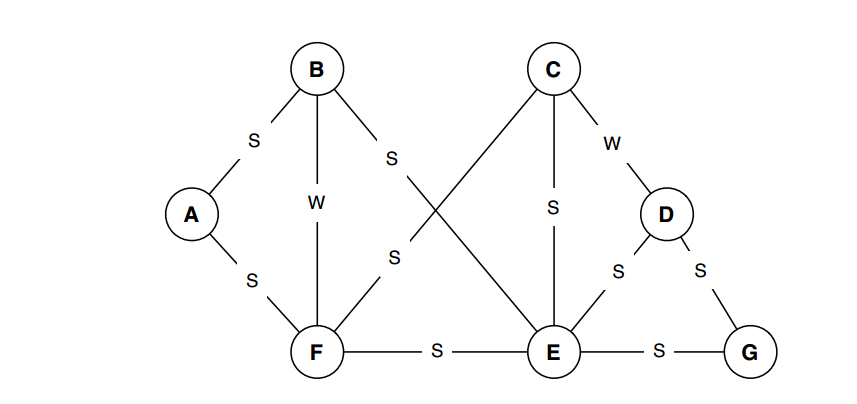
\includegraphics[width=15cm]{figures/figure1.png}
%\caption{A simple figure in \LaTeX. Reproduced from http://tinyurl.com/nqtrlj5 with the %permission of the copyright owner.}
%\label{fig:graph}
%\end{figure}
%
%\lipsum  % Replace with your text
%
%See Figure \ref{fig:graph}.
%
%
%\section{A Section that Contains a Table}
%
%\lipsum  % Replace with your text
%
%\begin{table}[ht]
%\center
%\begin{tabular}{cc|c}
%A & B & A XOR B\\
%\hline
%0 & 0 & 0\\
%0 & 1 & 1\\
%1 & 0 & 1\\
%1 & 1 & 0\\
%\end{tabular}
%\caption{A simple table in \LaTeX.}
%\label{tab:xor}
%\end{table}
%
%\lipsum  % Replace with your text
%
%This is shown in Table \ref{tab:xor}.
%
%
%\section{Summary}
%
%\lipsum  % Replace with your text
